% =====================================================================
\chapter{Introducción}
\label{cap:introduccion}

Los mercados financieros se mueven con la información. Un dato de inflación, un anuncio del
Banco Central o el resultado de una elección cambian lo que los inversores esperan de las
empresas, y esas expectativas se trasladan a los precios. Los medios económicos son uno de los
canales por los que esa información circula. Desde hace casi dos décadas, la literatura
financiera estudia si el sentimiento de esas notas ayuda a anticipar el comportamiento de las
acciones o si se limita a contar lo que el mercado ya hizo \citep{tetlock2007,garcia2013,verma2026}.

% ---------------------------------------------------------------------
\section{Problemática observada}

En la conversación cotidiana sobre la bolsa argentina está muy extendida la idea de que «las
noticias mueven las acciones». La observación tiene sustento intuitivo, porque los días de
noticias grandes, como los posteriores a una elección, son también días de movimientos fuertes
del S\&P~Merval. Pero esa coincidencia no dice qué vino primero: es posible que las noticias
muevan al mercado, y también que los medios cuenten lo que el mercado ya hizo.

Para separar esas dos posibilidades con datos hay que poder \textit{medir} el sentimiento de la
prensa económica argentina y \textit{relacionarlo}, en el tiempo, con el comportamiento de las
acciones. Para el mercado argentino no existía con qué hacerlo: ni un corpus ordenado de prensa
económica, ni un modelo de sentimiento entrenado para ese lenguaje, ni un índice diario de
tensión del mercado como el VIX de Chicago. El problema de este trabajo es, entonces,
metodológico: construir esa medición y ponerla a prueba con métricas de ciencia de datos.

En esta tesina, el \textit{shock informativo} del título se mide como \textbf{sentimiento
inesperado}: una rueda cuyas noticias son más positivas o más negativas que lo habitual en las
ruedas anteriores (sección~\ref{sec:inesperado}).

% ---------------------------------------------------------------------
\section{Hipótesis de investigación}
\label{sec:hipotesis}

\begin{quote}
\textbf{Hipótesis (H1).} Es posible construir una metodología de ciencia de datos que mida el
sentimiento de las noticias económicas argentinas y lo relacione con el comportamiento de las
acciones que cotizan en BYMA.

\textbf{Hipótesis nula (H0).} No es posible construir esa metodología: o el sentimiento no se
puede medir mejor que con un modelo genérico, o no se relaciona con el comportamiento de las
acciones en ninguna dirección.
\end{quote}

H0 es la negación exacta de H1. Para que la hipótesis no sea trivialmente verdadera, se fijó de
antemano, antes de ver los resultados, un \textbf{criterio de aceptación} con dos partes que se
tienen que cumplir a la vez:

\begin{enumerate}[label=\arabic*.]
  \item \textbf{Medir.} El modelo de sentimiento construido (FinBETO) clasifica las oraciones de
        noticias que nunca vio mejor que un modelo de sentimiento en español ya existente, medido
        con el F1 macro.
  \item \textbf{Relacionar.} En al menos una de las dos direcciones, un modelo predictivo que
        agrega la información del otro lado supera a uno que no la tiene, en ruedas que ningún
        modelo vio al entrenar:
        \begin{itemize}
          \item \textit{noticias \flecha{} precio}: el sentimiento ayuda a predecir si la acción
                sube en la rueda siguiente;
          \item \textit{precio \flecha{} sentimiento}: el mercado ayuda a predecir si el
                sentimiento de las noticias de la rueda siguiente es más positivo que lo habitual.
        \end{itemize}
        «Supera» quiere decir que el intervalo de confianza del 95\% de la diferencia de AUC entre
        los dos modelos queda entero por encima de 0 (sección~\ref{sec:criterio}).
\end{enumerate}

Las dos direcciones se prueban porque cualquiera de las dos es una relación entre noticias y
mercado. Lo que se esperaba de antemano, por la literatura \citep{tetlock2007,verma2026}, era que
las noticias no anticiparan el precio y que el precio sí anticipara el sentimiento de las notas.

% ---------------------------------------------------------------------
\section{Objetivos}

\textbf{Objetivo general.} Construir y evaluar una metodología de ciencia de datos que mida el
sentimiento de la prensa económica argentina y determine en qué dirección se relaciona con el
comportamiento de las acciones de BYMA.

Los objetivos específicos se plantean como resultados a obtener (tabla~\ref{tab:objetivos}).

\begin{table}[H]
\centering\small
\begin{tabularx}{\linewidth}{@{}C{0.9cm}YL{2.1cm}@{}}
\toprule
\textbf{Obj.} & \textbf{Resultado a obtener} & \textbf{Dónde} \\
\midrule
1 & Un corpus de noticias económicas argentinas depurado, con cada nota asignada a la primera rueda en la que el mercado pudo reaccionar a ella & Caps.~\ref{cap:datos} y~\ref{cap:preparacion} \\
2 & Un modelo de sentimiento para la prensa económica argentina, evaluado en noticias no vistas y comparado con un modelo existente & Cap.~\ref{cap:preparacion} \\
3 & Un conjunto de variables por acción y por rueda: sentimiento inesperado, sentimiento propio de cada empresa, retorno, volumen anormal y VIX argentino & Cap.~\ref{cap:preparacion} \\
4 & Un modelo predictivo evaluado en ruedas no vistas que indique si las noticias anticipan al mercado, si el mercado anticipa a las noticias, o ninguna de las dos cosas & Caps.~\ref{cap:modelado} y~\ref{cap:evaluacion} \\
\bottomrule
\end{tabularx}
\caption{Objetivos específicos. Fuente: elaboración propia.}
\label{tab:objetivos}
\end{table}

% ---------------------------------------------------------------------
\section{Antecedentes}
\label{sec:antecedentes}

\textbf{Noticias y precios.} \citet{tetlock2007} encontró, con una columna del \textit{Wall
Street Journal}, que la relación existe en las dos direcciones: el pesimismo anticipa bajas que
se revierten, y los retornos bajos anticipan más pesimismo. \citet{garcia2013} mostró que el
sentimiento anticipa los retornos casi solo en las recesiones. La cobertura importa por sí misma
\citep{fang2009,engelberg2011}, y trabajos recientes preguntan si las noticias influyen en el
precio o reflejan lo que ya tiene \citep{verma2026}, en qué momento lo incorpora
\citep{kargarzadeh2026} y si las notas de la noche explican el salto de apertura
\citep{glasserman2025}.

\textbf{Medición del sentimiento.} Se pasó de los diccionarios \citep{loughran2011} a los modelos
de lenguaje: FinBERT en inglés \citep{araci2019finbert} y, en español, BETO
\citep{canete2020beto}, MarIA \citep{gutierrez2022maria} y los modelos evaluados en titulares
económicos \citep{pan2023peerj}. A nivel de empresa, se clasifica el sentimiento hacia cada
entidad de la nota \citep{tang2023finentity}.

\textbf{Argentina y la región.} \citet{brana2016} clasificaron frases de noticias financieras
argentinas sin cruzarlas con precios; \citet{galdi2018} y \citet{cruzmontana2025} cruzaron
sentimiento y bolsa en Brasil y Colombia; \citet{coronado2022} probaron causalidad desde la
cantidad de noticias del COVID-19 hacia las bolsas de la región, y \citet{calandroni2026} estudió
el efecto de las elecciones sobre el Merval. No se encontró un trabajo que cruce el sentimiento de
la prensa económica argentina con las acciones de BYMA: ese es el vacío que cubre esta tesina.

% ---------------------------------------------------------------------
\section{Metodología: CRISP-DM}
\label{sec:metodologia}

Es un estudio observacional y longitudinal: sigue las variables durante \dato{dataset.ruedas}
ruedas, de mayo de 2025 a abril de 2026, y evalúa su relación con modelos predictivos. El trabajo
sigue las seis fases de CRISP-DM \citep{wirth2000crispdm,chapman2000}, que organizan tanto este
documento como las carpetas del proyecto (figura~\ref{fig:pipeline} y tabla~\ref{tab:crispdm}).
Se trabajó en Python con \texttt{transformers}, \texttt{spaCy}, \texttt{scikit-learn}
\citep{pedregosa2011} y \texttt{statsmodels} \citep{seabold2010}.

\begin{figure}[H]
\centering
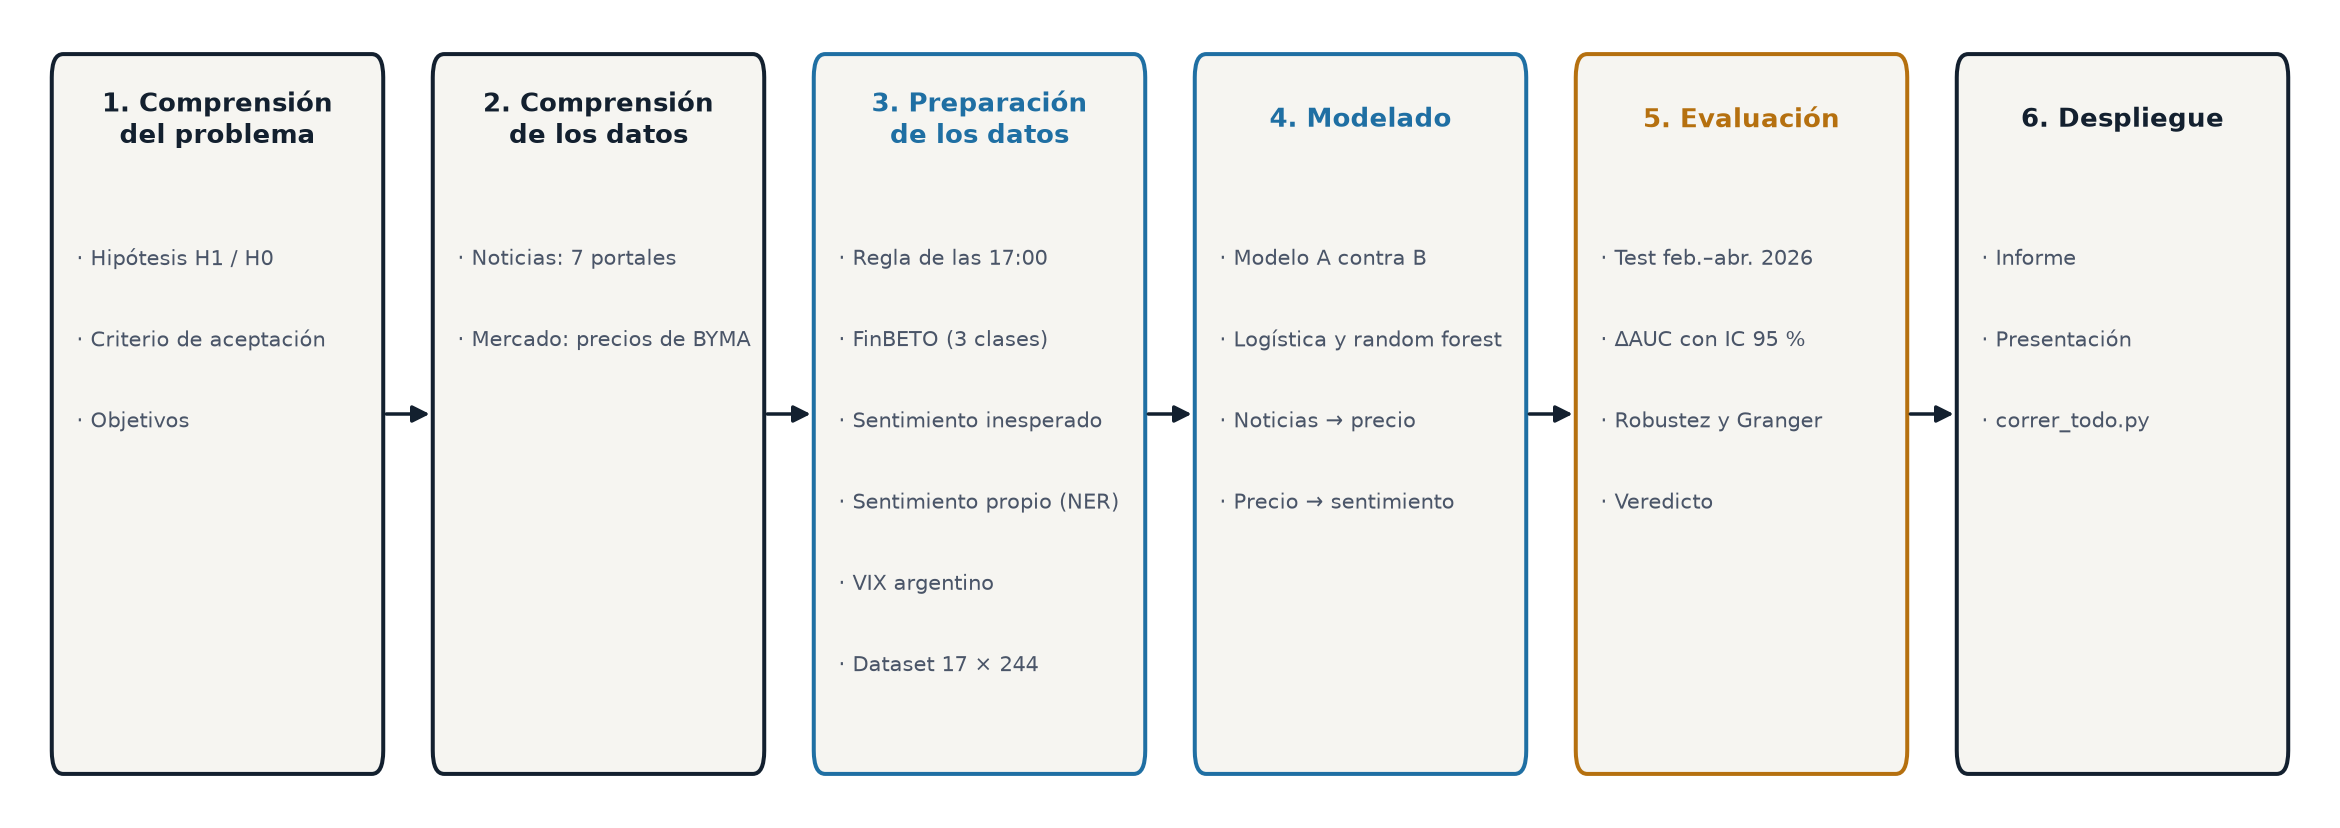
\includegraphics[width=\linewidth]{pipeline_crispdm.png}
\caption{El pipeline de la tesina, organizado según las seis fases de CRISP-DM. Las flechas siguen
el orden en que se ejecuta cada paso. Fuente: elaboración propia.}
\label{fig:pipeline}
\end{figure}

\begin{table}[H]
\centering\small
\begin{tabularx}{\linewidth}{@{}L{3.6cm}YL{1.9cm}@{}}
\toprule
\textbf{Fase de CRISP-DM} & \textbf{Qué se hace en esta tesina} & \textbf{Capítulo} \\
\midrule
1. Comprensión del problema & Hipótesis, criterio de aceptación y objetivos & \ref{cap:introduccion} y~\ref{cap:marco} \\
2. Comprensión de los datos & Recolección y auditoría de las noticias; panel de acciones & \ref{cap:datos} \\
3. Preparación de los datos & Cada nota a su rueda; etiquetado y FinBETO; sentimiento inesperado y propio; retorno, volumen anormal y VIX; dataset unificado & \ref{cap:preparacion} \\
4. Modelado & Modelo A contra B, regresión logística y random forest, corte temporal & \ref{cap:modelado} \\
5. Evaluación & Métricas en el test, robustez, verificación clásica y veredicto & \ref{cap:evaluacion} \\
6. Despliegue & Este informe, la presentación y la reproducibilidad del proyecto & Anexo~\ref{anx:repro} \\
\bottomrule
\end{tabularx}
\caption{Las fases de CRISP-DM en esta tesina. Fuente: elaboración propia.}
\label{tab:crispdm}
\end{table}

El trabajo se dividió en dos partes: el \textbf{lado de noticias} (corpus, sentimiento y
entidades), a cargo de Gino Frigoni, y el \textbf{lado bursátil} (panel de acciones y VIX
argentino), a cargo de Nicolás Diddi. Las fases de modelado y evaluación integran el trabajo de
ambos.

\textbf{Qué cambió respecto de la versión anterior.} Una versión previa de este trabajo contrastó
la relación con modelos VAR y pruebas de causalidad de Granger. Siguiendo la devolución de la
cátedra, la prueba de la hipótesis pasó a ser un modelo predictivo evaluado con métricas de
ciencia de datos (matriz de confusión, F1 y AUC) en ruedas no vistas. El VAR y Granger quedan como
verificación clásica en la sección~\ref{sec:verificacion}.
